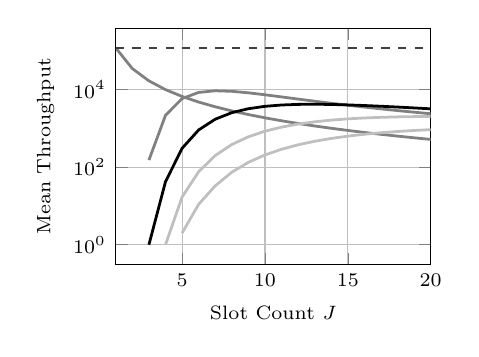
\begin{tikzpicture}
\begin{semilogyaxis}[
font=\scriptsize,
width=4cm,
height=3cm,
scale only axis,
xmin=1,
xmax=20,
xlabel={Slot Count $J$},
xmajorgrids,
ylabel={Mean Throughput},
ylabel near ticks,
ymajorgrids,
legend style={font=\tiny, at={(1,0)},anchor=south east, draw=black,fill=white,legend cell align=right}
]

\addplot [color=gray,solid,line width=1.0pt]
coordinates{
(1, 117955)
(2, 34614)
(3, 16724)
(4, 9944)
(5, 6631)
(6, 4756)
(7, 3588)
(8, 2810)
(9, 2264)
(10, 1865)
(11, 1565)
(12, 1333)
(13, 1150)
(14, 1003)
(15, 883)
(16, 783)
(17, 700)
(18, 630)
(19, 570)
(20, 518)
};
%\addlegendentry{$T$};

\addplot [color=gray,solid,line width=1.0pt]
coordinates{
%(1, 0)
%(1, 0)
%(2, 0)
(3, 152)
(4, 2158)
(5, 5824)
(6, 8417)
(7, 9267)
(8, 8992)
(9, 8222)
(10, 7318)
(11, 6447)
(12, 5669)
(13, 4997)
(14, 4423)
(15, 3936)
(16, 3522)
(17, 3168)
(18, 2865)
(19, 2603)
(20, 2375)
};
%\addlegendentry{$T=8$};


\addplot [color=black,solid,line width=1.0pt]
coordinates{
%(1, 0)
%(2, 0)
(3, 1)
(4, 42)
(5, 305)
(6, 907)
(7, 1718)
(8, 2529)
(9, 3202)
(10, 3687)
(11, 3989)
(12, 4138)
(13, 4171)
(14, 4120)
(15, 4013)
(16, 3870)
(17, 3705)
(18, 3531)
(19, 3353)
(20, 3178)
};
%\addlegendentry{$T=4$};

\addplot [color=lightgray,solid,line width=1.0pt]
  coordinates{
%(1, 0)
%(2, 0)
%(3, 0)
(4, 1)
(5, 17)
(6, 76)
(7, 199)
(8, 383)
(9, 605)
(10, 843)
(11, 1074)
(12, 1287)
(13, 1472)
(14, 1627)
(15, 1753)
(16, 1850)
(17, 1922)
(18, 1972)
(19, 2003)
(20, 2018)
};
%\addlegendentry{$T=2$};

\addplot [color=lightgray,solid,line width=1.0pt]
  coordinates{
%(1, 0)
%(2, 0)
%(3, 0)
%(4, 0)
(5, 2)
(6, 11)
(7, 33)
(8, 74)
(9, 133)
(10, 206)
(11, 289)
(12, 376)
(13, 464)
(14, 549)
(15, 629)
(16, 703)
(17, 769)
(18, 828)
(19, 880)
(20, 925)
};
%\addlegendentry{$T=1$};

\addplot [color=darkgray,dashed,line width=1.0pt,mark size=1.4pt]
  coordinates{
(1, 117955)
(2, 117955)
(3, 117955)
(4, 117955)
(5, 117955)
(6, 117955)
(7, 117955)
(8, 117955)
(9, 117955)
(10, 117955)
(11, 117955)
(12, 117955)
(13, 117955)
(14, 117955)
(15, 117955)
(16, 117955)
(17, 117955)
(18, 117955)
(19, 117955)
(20, 117955)
};

\end{semilogyaxis}
\end{tikzpicture}
